%%%%%%%%%%%%%%%%%%%%%%%%%%%%%%%%%%%%%%%%%%%%%%%%%%%%%%%%%%%%%%%%%%%%%%
%% ActionShap -- recommendation-only manuscript
%% Springer Nature template copied from the working SignalShap Overleaf package.
%% Compile with pdfLaTeX -> BibTeX -> pdfLaTeX -> pdfLaTeX.
%%%%%%%%%%%%%%%%%%%%%%%%%%%%%%%%%%%%%%%%%%%%%%%%%%%%%%%%%%%%%%%%%%%%%%

\documentclass[pdflatex,sn-mathphys-num]{sn-jnl}

\usepackage{graphicx}
\graphicspath{{figures/}}
\newcommand{\resdir}{tables}
\usepackage{multirow}
\usepackage{amsmath,amssymb,amsfonts}
\usepackage{amsthm}
\usepackage{mathrsfs}
\usepackage[title]{appendix}
\usepackage{xcolor}
\usepackage{textcomp}
\usepackage{manyfoot}
\usepackage{booktabs}
\usepackage{longtable}
\usepackage{array}
\usepackage{algorithm}
\usepackage{algorithmicx}
\usepackage{algpseudocode}
\usepackage{tikz}
\usetikzlibrary{arrows.meta,positioning,fit,backgrounds,calc}
\usepackage{microtype}
\hypersetup{pdftitle={ActionShap: Beyond Deletion Faithfulness toward Intervention-Robust Recommendation Explanations},pdfauthor={Mouad Louhichi; Redwane Nesmaoui; Mohamed Lazaar},pdfsubject={Intervention-grounded evaluation of recommendation explanations},pdfkeywords={explainable recommendation, intervention evaluation, Shapley value, faithfulness, actionability}}

\theoremstyle{thmstyleone}
\newtheorem{theorem}{Theorem}
\newtheorem{proposition}[theorem]{Proposition}
\newtheorem{corollary}[theorem]{Corollary}
\theoremstyle{thmstyletwo}
\newtheorem{example}{Example}
\newtheorem{remark}{Remark}
\theoremstyle{thmstylethree}
\newtheorem{definition}{Definition}

\newcommand{\safeinput}[1]{\IfFileExists{#1}{\input{#1}}{\ClassError{ActionShap}{Missing asset #1}{Upload the complete tables directory from the ActionShap Overleaf package.}}}
\newcommand{\AIA}{\operatorname{AIA}}
\newcommand{\NDCG}{\operatorname{NDCG}}
\newcommand{\Recall}{\operatorname{Recall}}
\newcommand{\MRR}{\operatorname{MRR}}
\newcommand{\LOO}{\operatorname{LOO}}
\raggedbottom

\begin{document}

\title[ActionShap]{ActionShap: Beyond Deletion Faithfulness toward Intervention-Robust Recommendation Explanations}

\author*[1]{\fnm{Mouad} \sur{Louhichi}}\email{mouad\_louhichi@um5.ac.ma}
\author[1]{\fnm{Redwane} \sur{Nesmaoui}}\email{redwane\_nesmaoui@um5.ac.ma}
\author[1]{\fnm{Mohamed} \sur{Lazaar}}\email{mohamed.lazaar@ensias.um5.ac.ma}
\affil*[1]{\orgdiv{National Higher School of Computer Science and Systems Analysis (ENSIAS)}, \orgname{Mohammed V University in Rabat}, \orgaddress{\city{Rabat}, \country{Morocco}}}
\date{}

\abstract{Recommendation explanations are commonly evaluated by deleting historical interactions, although deployed recommendation systems act through bounded changes to the influence of observed evidence. Deletion and feasible intervention therefore measure different properties. We introduce \textbf{ActionShap}, an architecture-agnostic protocol for history-conditioned recommenders with inference-time profile interventions. ActionShap separates deletion alignment, bounded-intervention alignment, and the quality of the joint action selected under a fixed budget. It fixes temporal splits, complete pre-test-history exclusion, target-plus-unseen-negative candidate sets, global tie priorities, signed action selection, abstention, convergence, and inference over distinct users. We evaluate Monte Carlo Shapley, locally weighted LIME, leave-one-out, greedy sequential deletion, and a random control on MovieLens-1M and Amazon Digital Music. The primary analysis uses a history-conditioned ItemKNN recommender, 1,000 users, five common seeds, and exact budget-two oracles; a latent profile model and full-unseen-catalogue subset provide robustness evidence. Shapley improves from deletion to bounded target-margin alignment in the primary ItemKNN conditions, but local methods retain higher absolute alignment and slightly better MovieLens NDCG decisions. The random control remains near its within-user null. ActionShap contributes an auditable evaluation instrument for separating perturbation sensitivity, absolute alignment, and intervention decision quality rather than claiming universal superiority for any explainer.}

\keywords{Explainable recommendation, Intervention evaluation, Faithfulness, Actionability, Shapley value, LIME}

\maketitle

\section{Introduction}
An explanation is often consumed as advice about where to act. A user, analyst, or system operator does not usually ask only whether a recommendation score changes when an input is deleted; they ask what will happen if a factor is discounted, suppressed, or otherwise modified within an available operating policy. The distinction is important in recommender systems because historical interactions are evidence, not necessarily controls. Removing an interaction can be a useful faithfulness diagnostic while being an unrealistic intervention.

This paper studies the resulting evaluation gap. We ask whether an attribution ranking predicts the effect of a feasible modification to the interaction history, and whether the explanation leads to a useful joint intervention under a fixed budget. The question is deliberately narrower than recourse: ActionShap does not claim that a user can cause a profile change, does not estimate causal effects in the world, and does not propose a new recommender architecture. It audits an explanation inside a frozen recommender and an explicitly declared intervention simulator.

The protocol is motivated by three observations. First, deletion and bounded modification are different estimands. A deletion moves a factor to a baseline that may be far outside an operational range. Second, pointwise attribution quality does not determine decision quality: a method can rank individual effects well while selecting a harmful pair, or select a good pair despite modest average rank agreement. Third, a method comparison is not interpretable without a chance control, valid-user counts, convergence diagnostics, and inference over distinct users rather than repeated seed--user records.

ActionShap addresses these issues with a history-conditioned interaction-player game. For each user, the most recent training interactions form the player set. A frozen ItemKNN model computes scores from the retained history at inference time, allowing masking and bounded downweighting to change the profile without retraining. The primary characteristic function is a continuous target-margin utility selected by an independent convergence study; NDCG@10 remains the operational ranking outcome. Every method receives the same temporal users, candidates, intervention strengths, action space, and tie rules.

Our contributions are fourfold:
\begin{enumerate}
  \item We formalize a recommendation-specific evaluation protocol that separates deletion faithfulness, bounded intervention, and budgeted decision quality under a frozen model.
  \item We provide complementary magnitude, signed-direction, success, abstention, regret, stability, and within-user null metrics, with explicit handling of constant vectors and inactive oracles.
  \item We give executable algorithms for paired Monte Carlo attribution, signed action selection, the exact $B\le2$ oracle, user-level inference, and independent convergence selection.
  \item We report a two-dataset, two-model, five-seed benchmark. The primary ItemKNN results show that Shapley can improve relative to deletion while LIME and LOO retain higher absolute alignment and downstream decision quality in some conditions.
\end{enumerate}

The paper makes no a priori claim that Shapley, LIME, LOO, or any other explainer is best. The framework is the contribution; method rankings are empirical and bounded by the declared offline simulator.



\section{Literature Review}
\subsection{Explainable recommendation}
Explainable recommendation includes feature, item, path, attention, sentiment, and natural-language rationales. Surveys emphasize that these forms serve different objectives, including user persuasion, model fidelity, transparency, and preference communication \cite{zhang2020survey}. Latent-factor explanations expose item or feature contributions, while post-hoc methods apply model-agnostic surrogates such as LIME and SHAP \cite{peake2018,nobrega2019,ribeiro2016,lundberg2017}. Sentiment- and phrase-level models construct explanations during recommendation rather than evaluating a post-hoc attribution \cite{zhang2014}. ActionShap addresses a complementary question: whether an explanation predicts the outcome of a declared feasible change.

\subsection{Recommender models and offline evaluation}
Classical matrix factorization and pairwise learning-to-rank remain foundations for offline recommendation \cite{koren2009,joachims2002,rendle2009,burges2005}. Neural collaborative filtering, recurrent session models, self-attentive sequence models, and bidirectional transformer recommenders broaden the architecture space \cite{he2017ncf,hidasi2016gru4rec,kang2018sasrec,sun2019bert4rec}. Graph recommenders introduce a further distinction between a trained graph representation and an inference-time profile intervention \cite{wang2019ngcf,he2020lightgcn}. We use ItemKNN as the primary model because its history dependence is transparent under masking; the profile aggregator is a robustness model, not a claim to cover all architectures.

Offline evaluation depends on temporal leakage, negative sampling, exposure, and the candidate universe. Results on a target-plus-negative set are sampled-ranking results, not catalogue retrieval. Evaluation choices can materially change rankings between methods and models \cite{harper2016,bennett2007,saito2021}. ActionShap fixes these choices before final testing, reports popularity references, and separates sampled ranking from full-unseen-catalogue evaluation.

\subsection{Faithfulness, counterfactual evaluation, and recourse}
Deletion and insertion tests measure model dependence but can be sensitive to the baseline and perturbation path. Sanity checks show that some attribution maps can appear plausible while failing model or data randomization tests \cite{adebayo2018}. Perturbation-based explanations also raise the question of whether the perturbation remains within a meaningful data manifold \cite{hooker2019}. Counterfactual recommendation and recourse methods instead search for profile or graph changes that alter a ranking or decision \cite{ghazimatin2020,tran2021,tan2021,yao2022,baklanov2024,barkan2024,gurevitch2025,mohammadi2025,nguyen2026,wachter2017,karimi2021}. ActionShap does not generate causal recourse. It evaluates an attribution under a fixed intervention policy and makes the policy, cost, authority, and offline limitations explicit.

\subsection{Interpretable machine learning and cooperative attribution}
Interpretability is not a single property: faithfulness, stability, simulatability, and usefulness can disagree \cite{gilpin2018,arrieta2020,molnar2022,samek2017,deyoung2020}. SHAP connects feature attribution with cooperative-game values, while sampling makes the construction applicable when exact enumeration is infeasible \cite{shapley1953,castro2009,lundberg2020,covert2021}. ActionShap treats Shapley as one interchangeable explainer. Its axioms do not imply causal validity, intervention feasibility, or decision superiority; these are measured separately.

\begin{table}[t]
\centering
\small
\caption{Positioning by evaluation target.}
\label{tab:positioning}
\begin{tabular}{lcccc}
\toprule
Approach & Explainer audit & Feasible policy & Joint regret & Abstention\\
\midrule
Deletion/insertion & Yes & No & No & No\\
Counterfactual explanation & Usually generates & Method-specific & Sometimes & Method-specific\\
Algorithmic recourse & No & Yes & Optimization target & Often\\
ActionShap & Yes & Yes & Yes & Yes\\
\bottomrule
\end{tabular}
\end{table}

\section{Background and Problem Formulation}
\subsection{Temporal user-specific game}
For user $u$, let $H_u^{\mathrm{train}}$ contain all interactions before validation and test. The player set is the most recent training window,
\begin{equation}
P_u=\{p_{u1},\ldots,p_{un_u}\},\qquad n_u\le n_{\max}=20,
\end{equation}
and define the older training context $B_u=H_u^{\mathrm{train}}\setminus P_u$. Interactions are ordered by $(\mathrm{timestamp},\mathrm{original\_record\_index})$; the last event is test and the preceding event is validation. Validation and test events are never players. Models are fitted using the complete training histories $H_u^{\mathrm{train}}$, but the released scoring implementation excludes older interactions $B_u$ from inference-time scoring: the profile score $f_u(i;S)$ depends only on $S$. Thus $B_u$ is not silently added as fixed scoring context. Consequently, $n_{\max}$ is both the operating profile boundary and the player-game boundary; the $n_{\max}\in\{50,100\}$ runs are sensitivity analyses of that boundary, not experiments that hold the recommender input fixed.

Every user has a fixed candidate set $E_u$ containing the held-out target and sampled negatives. Negatives exclude the complete pre-test history, including validation. The user seed, candidate seed, tie seed, model seed, and attribution seed are independent. Full-catalogue robustness uses the target plus all unseen items. Target coverage is one by construction and is not called retrieval recall.

\subsection{History-conditioned recommenders}
The primary ItemKNN score is a weighted mean of frozen item--item similarities:
\begin{equation}
f_u^S(i)=
\begin{cases}
\displaystyle\frac{\sum_{h\in S}w_hs(i,h)}{\sum_{h\in S}w_h},&S\ne\varnothing,\\[6pt]
0,&S=\varnothing.
\end{cases}
\end{equation}
A profile aggregator is used for robustness,
\begin{equation}
p_u(S)=
\begin{cases}
\displaystyle\frac{\sum_{h\in S}w_hq_h}{\sum_{h\in S}w_h},&S\ne\varnothing,\\[6pt]
\mathbf 0,&S=\varnothing,
\end{cases}
\qquad f_u^S(i)=q_i^\top p_u(S).
\end{equation}
Its item embeddings are trained once with a leave-one-out BPR-style objective and then frozen. Static user embeddings are excluded from attribution because post-training history masking cannot change their scores.

\subsection{Utilities and interventions}
The primary characteristic function is the target-margin utility
\begin{equation}
v_u^{\mathrm{attr}}(S)=\sigma\left(s_y^S-\frac{1}{L}\sum_{i\in\operatorname{TopL}_{-y}(S)}s_i^S\right),
\end{equation}
where $s_i^S:=f_u^S(i)$, $y$ is the temporal target, $L=10$, and $\sigma(t)=(1+e^{-t})^{-1}$ has unit temperature. The competitor set $\operatorname{TopL}_{-y}(S)$ is recomputed from the current coalition scores for every coalition $S$; it contains the ten highest-scoring candidates other than $y$. Every retained positive interaction starts with inference-time weight $w_h=1$. No temporal decay or rating-dependent weight is used. An action changes only these inference-time weights and never retrains the model. The operational ranking outcome is
\begin{equation}
q_u(S)=\NDCG@10(f_u^S,y).
\end{equation}
All effects and regrets are stored separately for target margin and NDCG. The empty coalition has target-margin utility $0.5$ and deterministic catalogue ties.

For an action $A\subseteq P_u$, let $P_u^{A,\rho}$ denote the same retained player window with weights
\begin{equation}
w_p^{A,\rho}=\begin{cases}\rho,&p\in A,\\1,&p\notin A,\end{cases}
\end{equation}
and define the signed intervention effect for either utility $z\in\{v_u^{\mathrm{attr}},q_u\}$ by
\begin{equation}
\Delta_u^z(A;\rho)=z_u(P_u^{A,\rho})-z_u(P_u).
\end{equation}
Deletion and bounded singleton effects are therefore
\begin{equation}
\Delta_{u,p}^{z,\mathrm{del}}=\Delta_u^z(\{p\};0),
\qquad
\Delta_{u,p}^{z,\mathrm{bnd}}=\Delta_u^z(\{p\};0.5).
\end{equation}
Deletion is the diagnostic $w_p\leftarrow0$. The primary feasible intervention is bounded downweighting,
\begin{equation}
\operatorname{do}(p;\rho):w_p\leftarrow\rho w_p,\qquad \rho=0.5,
\end{equation}
with $\rho=0.25$ as a predeclared sensitivity. No model retraining occurs after an intervention.

The action space is
\begin{equation}
\mathcal A_{u,B}=\{A\subseteq P_u:|A|\le B\},
\end{equation}
including no action. The primary scientific budget is $B=2$. A signed attribution predicts downweighting benefit as $-\phi$; only positive predicted benefit is selected. LOO is an algebraic deletion oracle at $B=1$, not a headline competitor.

\section{Methodology}
\subsection{Protocol architecture}
Figure~\ref{fig:architecture} summarizes the evaluation pipeline used throughout the paper. The architecture is placed with the methodology because it defines the sequence of player construction, scoring, attribution, intervention, and outcome measurement before the experimental results are introduced.

\begin{figure}[t]
\centering
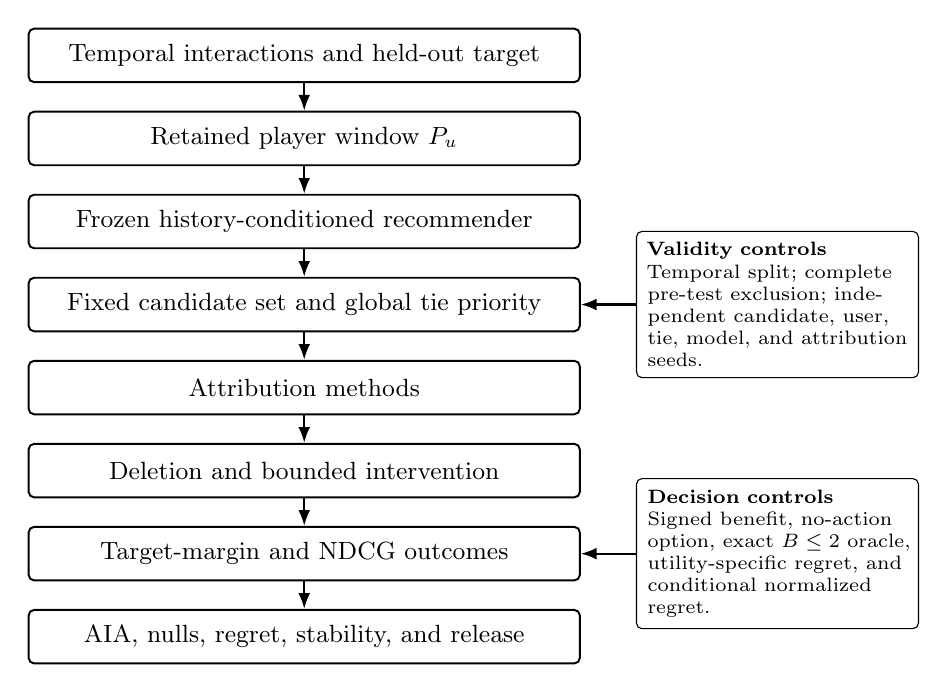
\begin{tikzpicture}[
  stage/.style={draw=black, fill=white, rounded corners=2pt, minimum width=7cm, minimum height=0.68cm, align=center, font=\small, line width=.7pt},
  edge/.style={-{Latex[length=2mm]}, draw=black, line width=.8pt},
  note/.style={draw=black, fill=white, rounded corners=2pt, align=left, font=\scriptsize, inner sep=4pt}
]
\node[stage] (a) {Temporal interactions and held-out target};
\node[stage, below=3.5mm of a] (b) {Retained player window $P_u$};
\node[stage, below=3.5mm of b] (c) {Frozen history-conditioned recommender};
\node[stage, below=3.5mm of c] (d) {Fixed candidate set and global tie priority};
\node[stage, below=3.5mm of d] (e) {Attribution methods};
\node[stage, below=3.5mm of e] (f) {Deletion and bounded intervention};
\node[stage, below=3.5mm of f] (g) {Target-margin and NDCG outcomes};
\node[stage, below=3.5mm of g] (h) {AIA, nulls, regret, stability, and release};
\foreach \x/\y in {a/b,b/c,c/d,d/e,e/f,f/g,g/h}{\draw[edge] (\x)--(\y);}
\node[note, right=7mm of d, text width=3.3cm] (v) {\textbf{Validity controls}\\Temporal split; complete pre-test exclusion; independent candidate, user, tie, model, and attribution seeds.};
\draw[edge] (v.west)--++(-4mm,0)|-(d.east);
\node[note, right=7mm of g, text width=3.3cm] (q) {\textbf{Decision controls}\\Signed benefit, no-action option, exact $B\le2$ oracle, utility-specific regret, and conditional normalized regret.};
\draw[edge] (q.west)--++(-4mm,0)|-(g.east);
\end{tikzpicture}
\caption{ActionShap evaluation architecture. The fixed vertical path separates player construction, model scoring, attribution, intervention execution, and outcome measurement. Side panels show controls held constant across methods.}
\label{fig:architecture}
\end{figure}

\subsection{Attribution methods}
For a sampled base permutation $\pi_m$, let $S_{p,\pi_m}$ be the predecessor coalition of player $p$. We use $M_{\mathrm{pair}}$ base permutations and also evaluate each reverse order, giving $T=2M_{\mathrm{pair}}$ total prefix walks. The estimator is
\begin{equation}
\widehat\phi_{u,p}=\frac{1}{T}\sum_{t=1}^{T}\left[v(S_{p,\pi_t}\cup\{p\})-v(S_{p,\pi_t})\right].
\end{equation}
The reverse orders are antithetic variance-reduction partners and coalition states are cached. In the executable configuration, \texttt{permutations} denotes $M_{\mathrm{pair}}=500$, hence $T=1000$ evaluated orders. The comparison includes locally weighted binary-mask LIME, LOO, greedy sequential deletion, and random attribution. No method observes measured intervention effects, oracle actions, or aggregate test outcomes.

For completeness, the greedy and random controls are defined operationally. Greedy sequential deletion starts at $S_0=P_u$. At step $t$ it evaluates $v_u^{\mathrm{attr}}(S_{t-1}\setminus\{p\})-v_u^{\mathrm{attr}}(S_{t-1})$ for every remaining player, selects the largest benefit, breaks ties by the lowest player index, records the signed value under the convention that $-\phi$ predicts downweight benefit, and recomputes the next step from the reduced coalition. It repeats until every player is ordered; it does not inspect bounded effects or the oracle, and the later signed action rule may abstain. Random attribution draws independent scores $r_{u,p}\sim\mathcal{N}(0,1)$ for every user and experiment seed using NumPy's seeded generator. The random vector is passed through the same signed action-selection rule as every explainer, including the same budget and abstention option. Its seed is independently offset from the model/attribution seed by $1{,}000{,}000+u$, so it is redrawn per user and seed.

\begin{algorithm}[t]
\caption{Greedy sequential-deletion baseline}
\label{alg:greedy-baseline}
\begin{algorithmic}[1]
\Require target-margin utility $v$, player set $P_u$
\Ensure signed ranking vector $\phi^{\mathrm{greedy}}_u$
\State $S\gets P_u$; recompute $v(S)$
\While{$S\ne\varnothing$}
  \State evaluate every $v(S\setminus\{p\})-v(S)$ for $p\in S$
  \State choose the maximum; break ties by lowest player index
  \State record its negative as $\phi^{\mathrm{greedy}}_{u,p}$; set $S\gets S\setminus\{p\}$
\EndWhile
\end{algorithmic}
\end{algorithm}

\begin{algorithm}[t]
\caption{Random attribution negative control}
\label{alg:random-baseline}
\begin{algorithmic}[1]
\Require user $u$, player count $n_u$, seed $s$
\Ensure random signed scores and optional action
\State draw $r_{u,p}\overset{\mathrm{iid}}{\sim}\mathcal{N}(0,1)$ for $p=1,\ldots,n_u$
\State apply the common signed downweight rule with budget $B$ and abstention
\State do not evaluate intervention effects before selecting the action
\end{algorithmic}
\end{algorithm}

\subsection{Metrics}
Magnitude AIA is
\begin{equation}
\AIA_u(g)=\operatorname{Spearman}(|\phi^g_{u,p}|,|\Delta^{\mathrm{attr}}_{u,p}|).
\end{equation}
Deletion AIA and bounded AIA are reported separately; their difference is the Actionability Gap. Signed alignment compares $-\phi$ with signed intervention effects. We also report direction accuracy, top-$k$ precision, realized effect, success, harm, abstention, and stability.

For each user and seed, $R=1{,}000$ within-seed permutations shuffle effect magnitudes across players. We first compute the observed AIA and its $R$ null draws within each seed; then we average the observed value and each matched null draw across the five seeds within user. Bootstrap and paired inference operate on these distinct-user summaries. We report null means, null 95th percentiles, plus-one permutation $p$-values, and valid-user counts. Constant vectors are missing, not imputed.

\subsection{Decision quality and regret}
For utility $z$, the exact budget-two oracle is
\begin{equation}
A_u^{*,z}=\arg\max_{A\in\mathcal A_{u,2}}\Delta_u^z(A),
\end{equation}
and the method action is $\widehat A_{u,g}$. Regret is
\begin{equation}
\operatorname{Regret}_u^z(g)=\Delta_u^z(A_u^{*,z})-\Delta_u^z(\widehat A_{u,g}).
\end{equation}
For a general budget $B$, the utility-specific feasible oracle is
\begin{equation}
A_u^{*,z}(B)=\arg\max_{A\subseteq P_u,\,|A|\le B}\Delta_u^z(A).
\end{equation}
At $B=2$ the released primary results exhaustively enumerate no action, all singletons, and all pairs. The archived $B=3$ sensitivity was produced with the declared greedy lower-bound search rather than exhaustive triples; it is retained only for joint-effect, success, and abstention sensitivity. No normalized-regret claim is made for $B=3$. Exhaustive triples would require at most $1+20+\binom{20}{2}+\binom{20}{3}=1351$ actions per user and are recommended for a future regenerated $B=3$ release.

For utility $z$, normalized regret is
\begin{equation}
\operatorname{NRegret}_u^z(g)=
\frac{\Delta_u^z(A_u^{*,z})-\Delta_u^z(\widehat A_{u,g})}
{\Delta_u^z(A_u^{*,z})},
\qquad \Delta_u^z(A_u^{*,z})>\varepsilon,
\quad \varepsilon=10^{-12}.
\end{equation}
It is averaged only over active-oracle users. Zero means an oracle-equivalent action; one means that the oracle improves the utility but the selected action achieves no improvement; values above one mean that the selected action is harmful. Values below zero are rejected by validation for the exact shared action space (up to floating-point tolerance); they would indicate an oracle or action-space inconsistency. The quantity is not clipped to one.

\begin{algorithm}[t]
\caption{Paired Monte Carlo attribution}
\label{alg:shapley}
\begin{algorithmic}[1]
\Require $u,P_u,v,M_{\mathrm{pair}}$, attribution seed
\Ensure $\widehat{\boldsymbol\phi}_u$
\State Initialise $\hat\phi_{u,p}\gets0$ for all $p\in P_u$
\For{$m=1$ to $M_{\mathrm{pair}}$}
\State Draw base order $\pi_m$ and its reverse; evaluate both cached prefix walks
\For{each consecutive pair $(S,S\cup\{p\})$}
\State $\hat\phi_{u,p}\gets\hat\phi_{u,p}+v(S\cup\{p\})-v(S)$
\EndFor
\EndFor
\State Divide by $T=2M_{\mathrm{pair}}$ and record finite/constant-vector flags
\end{algorithmic}
\end{algorithm}

\begin{algorithm}[t]
\caption{Signed action selection and exact budget-two oracle}
\label{alg:actions}
\begin{algorithmic}[1]
\Require $\hat{\boldsymbol\phi}_u$, profile weights, $\rho=0.5$, candidate set
\Ensure Method action and utility-specific oracle actions
\State Enumerate $\varnothing$, every singleton, and every pair
\For{each action $A$}
\State Apply $w_p\gets\rho w_p$ simultaneously for $p\in A$
\State Cache target-margin and NDCG effects
\EndFor
\State Select $\arg\max_A[-\sum_{p\in A}\hat\phi_{u,p}]$ over positive scores
\State Return $\varnothing$ when the best score is at most $10^{-12}$
\State Select the exact oracle separately for each utility
\end{algorithmic}
\end{algorithm}

\begin{algorithm}[t]
\caption{Distinct-user inference and AIA null}
\label{alg:inference}
\begin{algorithmic}[1]
\Require Five seed records per user and $R=1000$ null draws per seed
\Ensure User-level estimates and corrected comparisons
\For{each distinct user $u$ and seed $s$}
\State Compute seed-level AIA only for finite, nonconstant vectors
\For{$r=1$ to $R$}
\State Shuffle effect magnitudes within $(u,s)$; recompute the null AIA
\EndFor
\EndFor
\For{each distinct user $u$}
\State Average the observed AIA and each matched null draw across seeds
\EndFor
\State Bootstrap users; apply paired plus-one tests and Holm correction
\end{algorithmic}
\end{algorithm}

\begin{algorithm}[t]
\caption{Independent convergence selection}
\label{alg:convergence}
\begin{algorithmic}[1]
\Require $M_{\mathrm{pair}}\in\{25,50,100,250,500,1000\}$ and an independent $M_{\mathrm{pair}}=1000$ reference
\Ensure Selected $M_{\mathrm{pair}}$ or explicit unconverged status
\For{each candidate $M_{\mathrm{pair}}$}
\State Compare attribution ranks and signed-$B=2$ action Jaccard with the reference; each reported budget means twice as many evaluated orders
\State Record rank-valid fraction and threshold coverage
\EndFor
\State Select smallest $M_{\mathrm{pair}}$ with rank $\ge.95$, Jaccard $\ge.80$, rank validity $\ge.95$
\If{no candidate qualifies}\State Retain $M_{\mathrm{pair}}=1000$ as an unconverged stress test\EndIf
\end{algorithmic}
\end{algorithm}

\section{Experimental Protocol}
\subsection{Datasets and temporal split}
We use MovieLens-1M \cite{harper2016,ni2019} and Amazon Digital Music reconstructed from the Amazon Reviews 2018 release. Positive feedback is rating $\ge4$; Amazon duplicate user--item records retain the latest deterministic event and iterative 5-core filtering is reapplied after thresholding. MovieLens retains 6,035 users, 3,533 items, and 575,276 positive interactions. Amazon retains 10,623 users, 8,582 items, and 104,431 interactions. Source and processed hashes are recorded in the final manifest.

\subsection{Models, candidates, and gates}
The matrix includes ItemKNN and profile aggregation, five seeds, primary 1,000-user sampled ranking, 250-user full-catalogue subsets, and predeclared history, candidate, intervention-strength, budget, and utility sensitivities. ItemKNN uses cosine item--item similarities from binary training histories, removes self-similarity, retains the 200 largest non-zero neighbours per item, and applies no shrinkage or minimum-support threshold beyond the observed co-occurrence counts; all retained similarities are non-negative. The profile robustness model uses 64-dimensional item embeddings, ten leave-one-out BPR-style epochs, one sampled positive per user per epoch, uniform negatives outside the complete training history, learning rate $0.03$, and $L_2$ coefficient $10^{-4}$. Both models recompute the profile from the retained player window at inference time and are not retrained under an intervention.

The primary candidate set contains the target and 199 uniformly sampled unseen negatives. Candidate seed $1729$, user seed $2718$, tie seed $31415$, and model/attribution seeds $42$--$46$ are independent. The gate uses 200 users and a fixed 200-item sampled candidate set. ItemKNN passes all blocking masking gates. The profile model fails the NDCG masking threshold for one MovieLens seed (mean absolute change $0.000682$ versus $0.001$) and is retained as a nonblocking robustness boundary.

LIME uses 512 binary masks including the full, empty, and all leave-one-out masks, a normalized Hamming-distance kernel with width $0.25$, and ridge coefficient $1.0$. The target-margin competitor count is $L=10$ and the sigmoid temperature is one. The primary intervention is $\rho=0.5$; $\rho=0.25$ is sensitivity-only. The exact budget-two action space includes no action, all singletons, and all pairs.

\subsection{Statistical analysis}
For each seed we compute user-level quantities first; repeated seed values are then averaged within distinct user before bootstrap resampling. User bootstrap intervals use 10,000 draws, paired plus-one sign permutations use 10,000 draws, and the AIA null uses $R=1,000$ within-seed draws whose matched null values are averaged across seeds within user. Holm correction is applied within each experiment--metric comparison family. We report missing correlations, active-oracle counts, and conditional normalized regret. No coalition evaluation is an independent statistical observation.

\subsection{Reproducibility}
The real result archive contains 80 recommendation runs plus five convergence studies. All assets in this manuscript are generated from schema-v2 raw results with repository-relative paths and content hashes. The primary ItemKNN target-margin analysis uses $M_{\mathrm{pair}}=500$ base permutations and $T=1000$ evaluated orders; the independent convergence study selects lower diagnostic values for some conditions, while the conservative final floor is retained. The archived runs record macOS-26.5.1-arm64, Python 3.12.13, NumPy 2.4.6, SciPy 1.17.1, pandas 2.3.3, scikit-learn 1.9.0, matplotlib 3.11.1, and PyYAML 6.0.3. Historical processor model, RAM, and peak RSS were not serialized.

\section{Results}
All numerical claims below are generated only when \texttt{validation\_report.json} reports PASS. The legacy pilot is excluded from the canonical package.

\subsection{Recommendation quality and protocol audit}
Table~\ref{tab:recommendation-quality} shows that primary ItemKNN exceeds the popularity reference on both datasets. MovieLens ItemKNN reaches NDCG@10 $=0.284$ and HitRate@10 $=0.504$, compared with $0.158$ and $0.320$ for popularity. Amazon ItemKNN reaches $0.181$ and $0.285$, compared with $0.090$ and $0.155$. The profile model is weaker on both datasets and is therefore interpreted only as architectural robustness evidence.

Because each user has one held-out target, sampled-set HitRate@10 is numerically the same indicator as a one-target recall measure; HitRate is used here to avoid any implication of catalogue-level retrieval recall.

\safeinput{tables/recommendation_quality.tex}

\subsection{Faithfulness versus bounded alignment}
Table~\ref{tab:aia-components} separates deletion AIA, bounded AIA, and their difference. On MovieLens ItemKNN, Shapley has bounded AIA $0.779$ versus $0.933$ for LIME and $0.978$ for LOO. On Amazon, Shapley has bounded AIA $0.414$ versus $0.827$ and $0.851$. Thus Shapley does not win absolute alignment.

The contrast is in the change between perturbations. Shapley’s primary gap is $+0.0169$ on MovieLens and $+0.1285$ on Amazon. LIME and LOO are negative. The random control is close to zero and its confidence intervals include zero in the primary conditions. Greedy is negative on the primary conditions. The gap therefore measures a change of evaluation target; it is not an explanation-validity score.

\begin{figure}[t]
\centering

\includegraphics[width=\linewidth]{aia_components_robustness.pdf}
\caption{Deletion AIA, bounded-intervention AIA, and their difference for the five methods. Points are distinct-user means and intervals are user-bootstrap 95\% confidence intervals. Budget rows are excluded because budgets do not define singleton gap estimands.}
\label{fig:aia-components}
\end{figure}

\safeinput{tables/aia_components.tex}
\safeinput{tables/aia_permutation_null.tex}

\subsection{Joint intervention decisions}
The operational outcome is NDCG@10 under the exact $B=2$ action space. On MovieLens ItemKNN, LOO yields mean NDCG effect $0.0431$, LIME $0.0425$, and Shapley $0.0403$. Success is $28.9\%$, $28.8\%$, and $27.4\%$, respectively. Conditional normalized regret among 339 active-oracle users is $0.217$, $0.225$, and $0.268$. Local methods therefore retain a modest decision advantage on MovieLens.

On Amazon ItemKNN, NDCG effects are $0.0333$ for Shapley, $0.0331$ for LIME, and $0.0313$ for LOO. Conditional normalized regret among 196 active-oracle users is $0.206$, $0.197$, and $0.232$. The differences are small and do not support a universal winner. Random actions have negative mean NDCG effects on both datasets.

\safeinput{tables/intervention_outcomes.tex}

\begin{figure}[t]
\centering
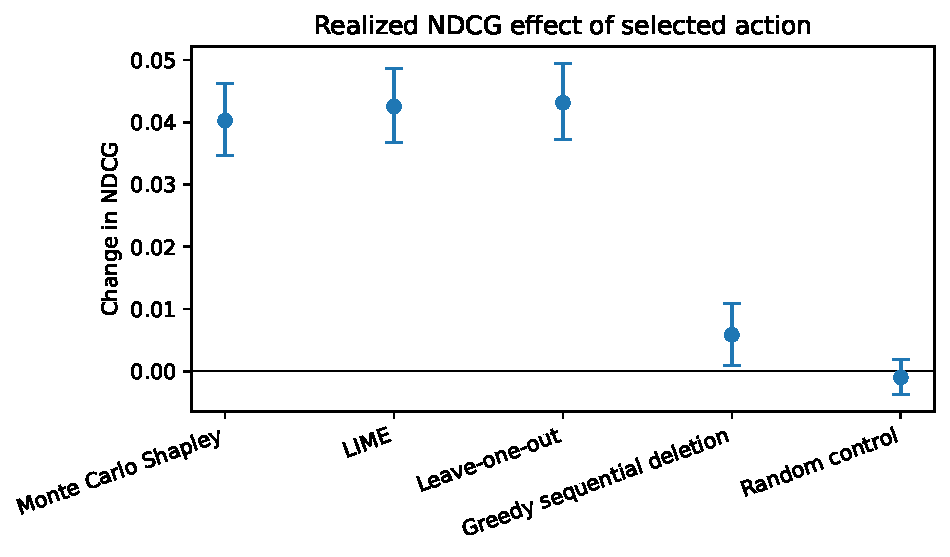
\includegraphics[width=\linewidth]{joint_ndcg_MovieLens-1M_itemknn_sampled_unseen_negatives_with_target_target_margin_primary_primary.pdf}
\caption{Primary MovieLens ItemKNN NDCG effect for actions selected at budget two. The comparison is retrospective and target-conditioned; intervals are distinct-user bootstrap intervals.}
\label{fig:joint-ndcg}
\end{figure}

\subsection{Null calibration and convergence}
The null-calibration table below reports the complete within-user null alongside the component table. The within-user AIA null is centred near zero for all primary ItemKNN conditions. Shapley, LIME, LOO, and greedy exceed the null for absolute AIA, while random attribution does not. This establishes that absolute alignment is not merely a consequence of the correlation statistic returning positive values.

Target-margin convergence selects $M_{\mathrm{pair}}=50$ for Amazon ItemKNN, $M_{\mathrm{pair}}=100$ for Amazon profile, $M_{\mathrm{pair}}=250$ for MovieLens ItemKNN, and $M_{\mathrm{pair}}=50$ for MovieLens profile; the final suite retains the conservative floor $M_{\mathrm{pair}}=500$ ($T=1000$ evaluated orders). Rank-valid fraction is the fraction of users with finite rank comparisons, whereas threshold coverage is the fraction of rank-valid users satisfying both the rank and action-overlap thresholds; coverage is diagnostic and is not a replacement for the rank-validity criterion. The NDCG attribution sensitivity remains unconverged at $M_{\mathrm{pair}}=1000$ and is reported only as a stress test.

\safeinput{tables/convergence.tex}
\safeinput{tables/attribution_stability.tex}

\begin{figure}[t]
\centering

\includegraphics[width=\linewidth]{convergence.pdf}
\caption{Independent Monte Carlo convergence against an $M_{\mathrm{pair}}=1000$ ($T=2000$ orders) reference. Efficiency is not used as a convergence criterion because the prefix walk telescopes.}
\label{fig:convergence}
\end{figure}

\subsection{Robustness and boundaries}
The positive Shapley gap persists across the primary ItemKNN candidate, history, intervention-strength, and full-catalogue conditions, but the absolute values vary. For Amazon full catalogue, the positive difference reflects reduced anti-alignment rather than positive bounded-intervention alignment: deletion AIA is $-0.2875$ and bounded AIA is $-0.1186$, so both absolute AIA values remain negative. Full-catalogue NDCG alignment is sparse and is treated descriptively. The longer-history conditions also show reduced masking sensitivity, supporting the use of $n_{\max}=20$ as a declared operating boundary rather than an arbitrary computational cap.

The profile model supplies a useful negative boundary: it can change rankings while underperforming popularity, and one MovieLens seed fails the NDCG masking threshold. This demonstrates why a non-degenerate masking gate and recommendation-quality audit are necessary before interpreting attribution results.


\subsection{Computational cost and release provenance}
Table~\ref{tab:computational-cost} reports the allocation-stage computational budgets. These are analytical scorer-call counts, not claims that every call has identical wall-clock cost; the exact ItemKNN batch implementation reuses cached similarity blocks, while the joint-action oracle is evaluated once per user and shared across methods.

\begin{table}[t]
\centering\small
\caption{Attribution-stage computational cost for a user with $n_u\le20$ players. Joint-action selection and the common exact oracle are excluded because they are shared outcome evaluations.}
\label{tab:computational-cost}
\begin{tabular}{@{}p{.22\textwidth}p{.23\textwidth}p{.43\textwidth}@{}}
\toprule
Method & Allocation-stage score budget & Reproducible definition \\
\midrule
Monte Carlo Shapley & $T(n_u+1)\le21{,}000$ prefix states before cache reuse & $M_{\mathrm{pair}}=500$ base orders plus reverses; coalition states cached and batched. \\
LIME & 512 binary masks & Full, empty, all leave-one-out masks, then seeded random masks; weighted ridge with Hamming kernel. \\
LOO & $n_u+1\le21$ states & Full coalition and every one-deletion coalition; exact deletion diagnostic. \\
Greedy deletion & $1+n_u(n_u+1)/2\le211$ states & Every remaining deletion is recomputed at every step; lower-index ties win. \\
Random control & 0 attribution utility calls & IID $\mathcal{N}(0,1)$ scores; the common action/effect evaluation is still applied after selection. \\
\bottomrule
\end{tabular}
\end{table}

The canonical artifact directory is \texttt{paper-ideas/ActionShap/paper-v3/}. The reproducibility command is:
\begin{verbatim}
python scripts/make_paper_assets.py --raw results/raw --out ../paper-v3
\end{verbatim}
The schema-v2 archive records total wall-clock duration for the 80 recommendation runs: the 60 ItemKNN runs range from approximately 29.8 to 2,851.6 seconds (mean 183.0 seconds), and the 20 profile runs range from approximately 26.9 to 299.6 seconds (mean 95.0 seconds). These are complete-pipeline durations rather than isolated explainer timings; the analytical call-budget table above is the comparable per-method cost measure. The archived runs record macOS-26.5.1-arm64, Python 3.12.13, NumPy 2.4.6, SciPy 1.17.1, pandas 2.3.3, scikit-learn 1.9.0, matplotlib 3.11.1, and PyYAML 6.0.3. Processor model, RAM, and peak RSS were not serialized in the historical schema-v2 files, so no unsupported hardware claim is inferred; the current runner records those fields for any regenerated release. The schema-v2 result archive SHA-256 is `ac4c7fb1993458b6b41054974ebff215710e7a8b5894c7aa6af828e94b2a5b0f`.

All paths in generated manifests are repository-relative and all release archives are verified by SHA-256. This manuscript package is versioned from source commit \texttt{d327160}; the schema-v2 result archive has SHA-256 \texttt{ac4c7fb1993458b6b41054974ebff215710e7a8b5894c7aa6af828e94b2a5b0f}. The source repository URL is https://github.com/mouadlouhichi/next-paper; its public visibility and any DOI-backed deposit are release actions outside the LaTeX package.


\section{Discussion and Broader Implications}
The results support a three-axis interpretation. LIME and LOO are strongest on absolute pointwise alignment because their constructions are local to deletion or the full profile. Shapley has lower absolute alignment but a larger positive change when the evaluation moves from deletion to bounded downweighting. This is consistent with coalition-context averaging, but the experiment does not establish a causal mechanism and the random control prevents interpreting the gap as standalone validity.

The decision results reinforce this distinction. On MovieLens, local methods select slightly better NDCG actions. On Amazon, Shapley and LIME are close, with modest differences in conditional regret. A method can therefore be more stable across perturbation semantics without selecting the best action for every operational utility. This is precisely why ActionShap reports pointwise alignment, signed direction, success, abstention, and regret together.

The protocol also clarifies what offline actionability means. The intervention is system-executable inside the frozen simulator: it changes an inference-time interaction weight without retraining. It is not automatically a user action, causal intervention, or prospective policy. A production deployment would need authority, cost, user-consent, and feedback-loop specifications that are outside this benchmark.

\subsection{Limitations and Threats to Validity}
\subsubsection{Construct validity}
Actionability is defined as predictive validity under one bounded downweighting policy. It is not perceived usefulness, legal recourse, user agency, or a causal effect in the world. All primary players are technically mutable, so feasibility does not differentiate factors; future work should study heterogeneous costs and user-side constraints.

\subsubsection{Metric validity}
NDCG is discrete and produces constant effect vectors for some users. We report missing correlations rather than imputing zero. Target margin is the converged attribution utility but has less direct operational meaning; NDCG is the action outcome and is never relabelled as target margin.

\subsubsection{Internal validity}
Temporal splitting and complete pre-test exclusion reduce leakage, but the audit remains target-conditioned. The held-out target defines the labelled instance being explained, which is appropriate for retrospective evaluation but unavailable to a prospective policy. Candidate sets are fixed and target coverage is one by construction; sampled ranking is not retrieval evaluation.

\subsubsection{External validity}
Two datasets and two history-conditioned models do not cover sequential transformers, graph recommenders, multimodal inputs, online feedback, provider objectives, or heterogeneous intervention costs. The full-catalogue subset is smaller than the primary cohort. The profile model’s quality shortfall and one failed gate are retained as explicit boundaries rather than generalized.

\section{Conclusion}
ActionShap provides a reproducible protocol for asking whether recommendation explanations predict the effects of feasible profile interventions. In the primary ItemKNN experiments, Shapley’s target-margin alignment improves relative to deletion, particularly on Amazon, while LIME and LOO retain higher absolute alignment and slightly better MovieLens NDCG decisions. The random control remains near its chance null, and a positive Actionability Gap is therefore not sufficient evidence of explanation validity. The principal contribution is the separation of deletion faithfulness, bounded-intervention alignment, and joint decision quality under a common, leakage-safe, abstention-aware protocol.



\backmatter

\section*{Declarations}
\textbf{Funding.} The authors declare that no funds, grants, or other support were received during the preparation of this manuscript.

\textbf{Competing interests.} The authors declare no competing interests.

\textbf{Ethics approval.} Not applicable. The study uses publicly available secondary recommendation data and involves no recruited human participants. Any future online or user study would require independent ethics review.

\textbf{Consent to participate / for publication.} Not applicable.

\textbf{Data availability.} MovieLens-1M was obtained from the GroupLens public release, and Amazon Digital Music was reconstructed from the Amazon Reviews 2018 public release after the documented rating threshold, deterministic deduplication, and iterative 5-core filtering. Source and processed-data SHA-256 values, split rules, and candidate construction are recorded in the final provenance manifest. The datasets are subject to their respective maintainers' terms and are not redistributed in this repository.

\textbf{Code and materials availability.} The canonical submission package is \texttt{paper-ideas/ActionShap/paper-v3/}. The raw experiment archive is distributed separately through the content-addressed release workflow because source datasets and raw JSON files are not ordinary manuscript assets.

\textbf{Author contributions.} M.L.: conceptualization, methodology, software, formal analysis, investigation, and writing---original draft. R.N.: methodology, validation, and writing---review and editing. M.Laz.: supervision, methodology, and writing---review and editing. All authors approved the final manuscript.


\appendix
% Explicit alphabetic appendix lettering: A--B are the only manuscript appendices.
\setcounter{section}{0}
\renewcommand{\thesection}{\Alph{section}}
\renewcommand{\thesubsection}{\thesection.\arabic{subsection}}
\renewcommand{\thetable}{\thesection\arabic{table}}
\setcounter{table}{0}
\section{Formal proofs and edge-case guarantees}\label{app:proofs}

\subsection{Efficiency of the prefix-walk estimator}
For any permutation $\pi=(p_1,\ldots,p_n)$, define $S_0=\varnothing$ and $S_j=\{p_1,\ldots,p_j\}$. The prefix-walk contribution of $p_j$ is $v(S_j)-v(S_{j-1})$. Consequently,
\begin{equation}
\sum_{j=1}^{n}\left[v(S_j)-v(S_{j-1})\right]=v(P_u)-v(\varnothing).
\end{equation}
Averaging over paired permutations preserves the identity up to floating-point arithmetic. The efficiency residual in the release is therefore a cache and arithmetic diagnostic, not a convergence criterion.

\subsection{Leave-one-out ceiling}
For deletion at $\rho=0$, $\Delta^{\mathrm{del}}_{u,p}=v(P_u\setminus\{p\})-v(P_u)$ and $\phi^{\mathrm{LOO}}_{u,p}=v(P_u)-v(P_u\setminus\{p\})$. Thus $|\phi^{\mathrm{LOO}}_{u,p}|=|\Delta^{\mathrm{del}}_{u,p}|$ for every valid nonconstant user and deletion AIA is one. LOO's deletion-to-bounded gap is consequently bounded above by zero; it is retained as a diagnostic oracle, not a positive-gap competitor.

\subsection{Exact budget-two action space}
With $n_u\le20$, the exact action space contains $1+n_u+\binom{n_u}{2}\le211$ actions, including no action. Each action is evaluated against target margin and NDCG using the same cached candidate scores. The oracle is therefore exact for every primary user and does not rely on a sampled action subset.

\section{Complete experimental contract}\label{app:contract}
\setcounter{table}{0}

\begin{table}[t]
\centering\scriptsize
\caption{Frozen experimental contract used for every paper-eligible run. The executable YAML and scripts are the source of truth; this table records every parameter that changes the estimand or reported uncertainty.}
\label{tab:contract}
\resizebox{\linewidth}{!}{%
\begin{tabular}{lll}
\toprule
Element & Primary setting & Robustness/sensitivity settings\\
\midrule
Datasets & MovieLens-1M; Amazon Digital Music, rating $\ge4$ & same\\
Temporal split & last test, penultimate validation; timestamp/index ties & complete pre-test exclusion\\
Model fitting & complete training histories & no retraining under intervention\\
Player/scoring history & most recent $n_{\max}=20$; older $B_u$ not scored & $n_{\max}\in\{50,100\}$\\
ItemKNN & cosine co-occurrence; top 200 non-zero neighbours; no shrinkage & same\\
Profile model & 64 dimensions; 10 BPR-style epochs; $\eta=.03$; $L_2=10^{-4}$ & robustness-only\\
Candidates & target + 199 uniform unseen negatives & 100, 500, full unseen catalogue\\
Tie/candidate/user seeds & 31415 / 1729 / 2718 & fixed across methods and five model seeds\\
Attribution utility & target margin, $L=10$, unit-temperature sigmoid & NDCG stress test\\
Shapley sampling & $M_{\mathrm{pair}}=500$, $T=1000$ reverse-paired orders & convergence $M_{\mathrm{pair}}\in\{25,50,100,250,500,1000\}$\\
LIME & 512 masks; Hamming kernel width .25; ridge $\alpha=1$ & same\\
Intervention & simultaneous downweight $w_p\leftarrow.5w_p$ & deletion and $\rho=.25$\\
Budget/oracle & exact all actions up to $B=2$, including no action & $B=1$ and $B=3$ joint decisions\\
Null/inference & $R=1000$ matched null draws; 10,000 bootstrap/permutation draws & Holm correction\\
\bottomrule
\end{tabular}}
\end{table}

The profile optimizer samples one positive item per user per epoch, excludes that positive from its temporary context, and samples a negative uniformly outside the user's complete training history. ItemKNN has no latent user embedding, shrinkage coefficient, minimum-support cutoff, or negative-similarity branch: the retained similarity matrix is non-negative by construction. AIA is Spearman rank correlation and is missing for constant or non-finite vectors. Normalized regret uses $\varepsilon=10^{-12}$ and is averaged only over positive-oracle users. The release archive records the exact dependency versions, source hashes, run durations, and selected users; complete per-user vectors remain in the compressed machine-readable asset rather than in the PDF.


\bibliography{actionshap-bibliography}

\end{document}
